%% LaTeX_Thesis_Template.tex
% An unofficial LaTeX template for Cranfield theses.

%%
% This document is an example of the use of the unofficial "cranfieldthesis" 
% LaTeX style file.  I hope it's useful, and good like.

%% Options for the bibliography generator
%% \bib_opts[bib_file]{library.bib}
%% \bib_opts[output_file]{bibliography.tex}

\documentclass[12pt, oneside]{book}

\usepackage{luatex85}

% Use the custom "cranfieldthesis" LaTeX style file. 
\usepackage{cranfieldthesis}
\usepackage{amssymb}
\usepackage{geometry}
\usepackage[titletoc]{appendix}
\usepackage{multirow}
\usepackage{tabularx}
\usepackage{lscape}
\usepackage{pdflscape}
\usepackage{rotating}
\usepackage{titletoc}
\usepackage{tikz}
% \usepackage{import}
\usepackage{float}
\usetikzlibrary{shapes, arrows, matrix}

\usepackage{scrlayer}

\DeclareNewLayer[
background,
rightmargin,
contents={%
	\parbox[b][\layerheight][c]{\dimexpr\footskip+\footheight\relax}{%
		\hfill\rotatebox{90}{\pagemark}}}
]{lscape.foot}

\DeclareNewLayer[
background,
textarea,
addhoffset=\dimexpr-\headsep-\headheight\relax,
width=\dimexpr\headsep+\headheight\relax,
%contents={\hfill\rotatebox{90}{\headmark}\hspace*{\headsep}}
contents={}
]{lscape.head}

\DeclareNewPageStyleByLayers{lscape}{lscape.foot,lscape.head}

\newcolumntype{b}{X}
\newcolumntype{s}{>{\hsize=.5\hsize}X}
\newcommand{\heading}[1]{\multicolumn{1}{c|}{\textbf{#1}}}

% By default, LaTeX uses a serif font - these are traditionally thought to be
% easier to read.   If you'd prefer sans-serif, please uncomment the 
% following line.
%\renewcommand{\familydefault}{\sfdefault}
\renewcommand{\rmdefault}{phv} % Arial
\renewcommand{\sfdefault}{phv} % Arial

\let\oldappendices\appendices
\let\endoldappendices\endappendices

\renewenvironment{appendices}{
	\oldappendices
		
	\addtocontents{toc}{\protect\setcounter{tocdepth}{1}}
	\renewcommand\thesection{\Alph{section}}%
	
	\titlecontents{section}
	[1.0em]
	{}
	{\appendixname~\thecontentslabel~}
	{}
	{\titlerule*[0.3pc]{.}\contentspage}
	
	\titleformat{\section}{\large\bfseries}{\appendixname~\thesection}{0.5em}{}
	\titleformat{\subsection}{\normalsize\bfseries}{\thesubsection}{0.5em}{}
	\titleformat{\subsubsection}{\normalsize\bfseries}{\thesubsubsection}{0.5em}{}
}{
	\endoldappendices
}

% Switch [1] for 1. in Reference list but maintain [1] in citation


\makeatletter\renewcommand{\@biblabel}[1]{#1.}\makeatother

% Example parameters for a typical taught MSc course
\title{A Web Based Terrain Modeller using Fractals and CAD}
\author{Miguel Marques}
\date{August 2016}
\school{Aerospace, Transport and Manufacturing}
\course{Computational and Software Techniques in Engineering \\ Digital Signal and Image Processing}
\degree{MSc}
\academicyear{2015--2016}
\supervisor{Dr Peter Sherar}
\copyrightyear{2016}


\begin{document}


%% Front matter
%
% This is where we do the title page, etc.
%

\frontmatter

% Standard-Form Title Pages
\maketitle

\pagestyle{plain}

% Abstract and Keywords
\begin{abstract}
    Type your abstract here.

	\subsubsection*{Keywords}
	Procedural Generation; Terrain Modelling; 
\end{abstract}

% Acknowledgements
\chapter{Acknowledgements}
The author would like to thank \dots

% Table of Contents
\sstableofcontents

% List of Figures
\sslistoffigures

% List of Tables
\sslistoftables

% List of Equations
\sslistofequations

% The list of abbreviations can't be automatically generated so you need to populate it yourself
\begin{listofabbreviations}
    \abbrev{fBm}{Fractional Brownian Motion}
    \abbrev{PMHCI}{Picewise Monotone Hermite Cubic Interpolation}
    \abbrev{HPF}{High-pass Filter}
    \abbrev{FFT}{Fast Fourier Transform}
    \abbrev{IFFT}{Inverse Fast Fourier Transform}
\end{listofabbreviations}


%% Main Matter
%
% This is where we include the main thesis content.
%
\mainmatter

\chapter{Introduction}
This is a sample of thesis text. This is a sample of thesis text. This is a 
sample of thesis text. This is a sample of thesis text. This is a sample of
thesis text.

This is a sample of thesis text. This is a sample of thesis text. This is a 
sample of thesis text. This is a sample of thesis text. This is a sample of
thesis text.

\chapter{Literature Review}

Procedural generation of terrains has been the focus for many graphics researchers for some time now. Through the years this research has been mostly based on fractional Brownian motion and its similarity to a skyline of mountains, first noticed by Mandelbrot in \cite{Mandelbrot1983}. 

% TODO: Document organization

% TODO: Fractal Dimension
% TODO: Hurst Exponent
% TODO: Self-similarity
% TODO: Self-affinity

\subsection{Fractal Dimension}

\begin{quotation}
	"A fractal is by definition a set for which the Hausdorff Besicovitch dimension strictly exceeds the topological dimension." \cite[p.15]{Mandelbrot1983}
\end{quotation}

The Hausdorff Besicovitch dimension, also called fractional or fractal dimension, is a measure used to characterize a fractal. This dimension $ D_f $ does not need to be an integer and, for a surface in $ \mathbb{R}^n $, $ D_f \in [n, n+1)$.

\subsection{Fractional Brownian Motion}

Fractional Brownian Motion (fBm) was introduced by Mandelbrot and van Ness in \cite{Mandelbrot1968} and it is an extension of Brownian Motion that uses the Hurst Exponent ($H$) as a parameter to control the correlation between successive values, such that, $ 0 < H < 1 $. More specifically if $H = 0.5$ then fBm is just normal Brownian Motion and, due to that, the increments are independent and not correlated; if $H > 0.5$ the increments have positive correlation and this results in smooth curves while if $H < 0.5$ the increments have negative correlation and this results in erratic curves. \cite{Musgrave1993}

In the field of fractal terrain generation fBm is approximated by $1/f^\beta$ noise, where $\beta$ is the spectral exponent of the noise. Considering $D_f$ as the fractal dimension and $D_E$ as the Euclidean dimension, $1/f^\beta$ noise follows the following rule:
\[
D_f = D_E + 1 - H = D_E + \frac{3-\beta}{2}
\]

\section{Terrain Modelling}

In this section the different methods used for terrain generation are analysed. All the analysed methods try to approximate fBms and they are divided in six categories:
\begin{itemize}
	\item Poisson Faulting
	\item Subdivision Methods
	\item Fourier Filtering
	\item Successive Random Additions
	\item Noise synthesis
	\item Generalized Stochastic Subdivision
\end{itemize}

%\begin{quotation}
%	"the small spectral sums used to create random fractals for computer graphics allow the character of the basis function to show through clearly in the result. Usually, the choice of basis function is implicit in the algorithm: it is a sine wave for Fourier synthesis, a sawtooth wave in polygon subdivision, and a piecewise-cubic Hermite spline in noise-based procedural fBm. You could use a Walsh transform and get square waves as your basis. Wavelets (Ruskai 1992) promise to provide a powerful new set of finite basis functions. And again, sparse convolution (Lewis 1989) or fractal sum of pulses (Lovejoy and Mandelbrot 1985) offer perhaps the greatest flexibility in choice of basis functions." \cite[pg 497]{Ebert2003}
%\end{quotation}

\subsection{Poisson Faulting}

The Poisson Faulting technique, also known as Random cuts algorithm, consists in applying Gaussian random displacements to a plane at Poisson distributed intervals. \cite{Musgrave1989}. This method was initially applied by Mandelbrot in \cite{Mandelbrot1983}. Although this method has the advantage of working for both planes and spheres, in the creation of random planets, it is $O(n^3)$ complex in time.

\subsection{Subdivision Methods}

The methods presented in this section derive from the midpoint displacement algorithm that consists in successively subdividing a line and displacing the division points. These methods are classified in two categories \cite{Mandelbrot1988}:
\begin{itemize}
	\item Wire-frame Midpoint Displacement
	\item Tile Midpoint Displacement
\end{itemize}

\subsubsection{Wire-frame Midpoint Displacement} \label{sect:wireframeMD}

In this type of methods the surface is thought of as a wire-frame mesh and the displacements are applied to the midpoints of the edges. This is the case of the Carpenter's Method \cite{Fournier1982} in which the wire-frame forms triangles which are recursively subdivided until there is no triangle with a side bigger than a specified length. Wire-frame methods are context independent as the only inputs that impact the shape of the generated surface come from the altitude values at the vertices. This context independence is the opposite of what happens with fBm, which incorporate an infinite span of context dependence \cite{Mandelbrot1988}.


% TODO: Talk about creases
%\begin{quotation}
%"The "creases" sometimes encountered in stochastic subdivision can be related to the displacement noise variances and to the absence of autocorrelation information in Markovian subdivision."\cite{Lewis1987}
% \end{quotation}

\subsubsection{Tile Midpoint Displacement}

In tile midpoint displacement methods the surface is seen as a collection of tiles and the displacements are applied to points in the middle of every tile. This methods are context dependent.

\paragraph{Triangular tile midpoint displacement}
In \cite{Mandelbrot1988} Mandelbrot proposes a method of tile displacement with triangles. In contrast with the Carpenter's method (section \ref{sect:wireframeMD}), the displacement is applied to the midpoint of the triangles using: \[ H(P) = \frac{H(A) + H(B) + H(C)}{3} + rand \] where $A$, $B$ and $C$ are the triangle vertices, $P$ is the triangle midpoint  and $rand$ is the random displacement value.

\paragraph{Diamond-Square Algorithm}
The Diamond-Square algorithm \cite{Fournier1982} consists in the subdivision of quadrilaterals in two steps: in the first step, known as diamond, the midpoint of the square is displaced using a random value; in the second step, known as square, the midpoint of the original square sides are interpolated from the value of the two square vertices and the two closest diamond vertices and displaced by another random value. In practice this is a hybrid between wire-frame and tile displacement method as when the initial structure is composed of squares it is not enough to just displace the tiles midpoints but also interpolate the edges midpoints.


\paragraph{Square-square subdivision}
In \cite{Miller1986} Miller proposes a method adapted from the CAD/CAM field. This method, denominated Square-Square subdivision, generates new points that form a square which is half the size of the existing one using the proportions 9:3:3:1, in which the nearest points have the greater weight. 


\paragraph{Hexagonal tile midpoint displacement}
In \cite{Mandelbrot1988} Mandelbrot also proposes the use of hexagonal tiles in the displacement method. This was due to his belief that the nesting properties of the displacement methods, that is when the generated points are nested in the old structure, was the cause of the creasing effect. Given the hexagon's properties, a structure like this will never nest but, instead, will create a crumpled boundary that fails to catch the eye, contrary to the "creases" that stand out.

% NB: Solves creases

\subsection{Fourier Filtering}

Another method to generate fBm surfaces is using the Inverse Fourier Transform. This is done by generating a two dimensional Gaussian white noise signal, applying a $1/f^\beta$ low-pass filter in the frequency domain, and using the result of the Inverse Fourier Transform of the filtered signal as a height field \cite{Musgrave1989}. % This method has a time complexity $O(n \log{n})$ 

\subsection{Successive Random Additions}

The Successive Random Additions algorithm \cite{Saupe1988} builds on top of the midpoint displacement algorithm. If old points are reused in subsequent phases of subdivisions, they are displaced with a random variable with an appropriate distribution \cite{Musgrave1989}. In terms of complexity this method is comprised of approximately twice the number of additions of the midpoint displacement algorithm \cite{Voss1985}.

\subsection{Noise synthesis}

Noise synthesis consists in the addition of successive frequencies of tightly band-limited noises \cite{Musgrave1989}. This can be done using several noise algorithms, such as, Perlin Noise \cite{Perlin1985}, Simplex Nosie \cite{Perlin2002} or OpenSimplex Noise \cite{Spencer2015}.

\subsection{Generalized Stochastic Subdivision}

% TODO:		- Generalized Stochastic
All the methods previously presented have a basis function that is, usually, implicit in the generation algorithm. This basis function can affect the final surface in different ways: the saw-tooth wave in polygon subdivision methods explains the creasing effect and the sine wave in Fourier synthesis causes the terrains to become periodic. In \cite{Lewis1987} Lewis proposes a method that interpolates several local points based on a autocorrelation function \cite{Musgrave1993}, that is, this algorithm is able to generate surfaces with any basis function.

% \subsubsection{Multifractals}
% TODO: 	- Multifractals

%\begin{quotation}
%	"Multifractals may be heuristically defined as "fractals that require a multiplicity of measures, such as fractal dimension, to characterize them." Another heuristic definition is "heterogeneous fractals, the heterogeneity of which is invariant with scale. They are most easily thought of as fractals whose dimension varies with location; the key point is that they are heterogeneous -- not the same everywhere"\cite{Musgrave1994}
%\end{quotation}

%See \cite{Evertsz1992}.

% TODO: Erosion

% \section{Constrained Terrain Generation}

\section{Terrain Representation}

% TODO: TINs

\subsection{Heigh field}
The height field, in some literature denominated as height map, is one of the most used forms of representing terrains in Computer Graphics. A height field stores an altitude value at regular intervals using a two-dimensional array \cite{Ebert2003}, and, as such, can be saved as a grayscale image. Due to the fact that only one altitude value is retained for a pair of coordinates this method can only represent surfaces, that is, it does not support overhangs or caves. 

%\subsubsection{DEM file format}
% TODO: DEM
% TODO: Vector map
% TODO: DTM

%\begin{quotation}
%	"There are several common file formats for height field data. There is the DEM (digital elevation map) format of the U.S. Geological Survey (USGS) height fields, which contain measured elevation data corresponding to the "quad" topographic [...]" \cite[pg 494]{Ebert2003}
%\end{quotation}

% \section{Terrain Rendering}

% TODO: Rendering Optimizations (GPUGems article)
% TODO: Scene Management
% TODO: Lighting
% TODO: Shadows
\chapter{Methodology} \label{chap:methodology}

\begin{notes}
	\item Write Chapter Introduction
\end{notes}

\section{Process Overview}

\begin{figure}[h!]
	\begin{center}
		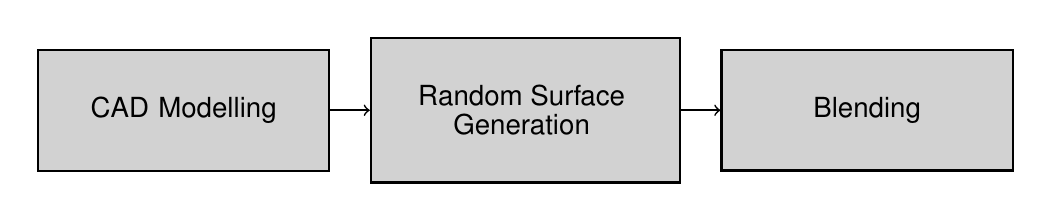
\begin{tikzpicture}[
		font=\sffamily,
		every matrix/.style={column sep=0.5cm, row sep=0.5cm},
		phase/.style={draw, thick, align=center, fill=gray!35, inner sep=.6cm},
		to/.style={->,semithick,font=\sffamily\footnotesize},
		every node/.style={anchor=center}
		]
		
		\matrix[matrix of nodes,ampersand replacement=\&]
		{
			|[phase, text width = 2.5cm] (1)| \shortstack{CAD Modelling} \& 
			|[phase] (2)| \shortstack{Random Surface \\ Generation} \& 
			|[phase, text width = 2.5cm] (3)| \shortstack{Blending} \\
		};
		
		\draw[to] (1) -- (2);
		\draw[to] (2) -- (3);
		\end{tikzpicture}
	\end{center}
	
	\caption{Process Phases}
	\label{fig:process_phases}
\end{figure}

The proposed workflow consists of three high level phases which are presented in Figure \ref{fig:process_phases}. The first is the CAD modelling phase (section \ref{sec:methodology:phase1}) which consists on the creation of a simplified model of the terrain, which will be denominated as base surface, containing only the main characteristics, such as, mountains and valleys. The second phase (section \ref{sec:methodology:phase2}) consists in the generation of the random surface from which the details will be acquired. Finally the third and final phase is the blending phase (section \ref{sec:methodology:phase3}) in which the base surface is combined with the random surface to create a more detailed version of the terrain.

\section {Phase 1: CAD Modelling} \label{sec:methodology:phase1}

The purpose of the CAD Modelling phase is to enabled the user to specify the main features of the terrain, such as mountains and valleys, using manual modelling. This phase results in the generation of a height map that contains the base surface.

\section{Phase 2: Random Surface Generation} \label{sec:methodology:phase2}

With the base surface obtained from the first phase it is now possible to generate a random surface with the same dimensions. This can be done using several methods, as discussed in Chapter \ref{chap:literature_review}. For the purpose of this application the chosen methods were Fourier Filtering (section \ref{sec:methodology:fourier}) and Noise Synthesis (section \ref{sec:methodology:noise}).


  \subsection{Fourier Filtering} \label{sec:methodology:fourier}
    
    The fourier filtering method, shown in Figure \ref{fig:fourier_filtering}, consists in applying a $f^{-\beta}$ filter to a white noise surface in frequency domain. 
    
    This method only needs one parameter, the filter power ($\beta$).
    
    Using a fork and join approach it is possible to parallelize this method as there is a parallel version of each of it's steps.
    
    
    \begin{figure}[!h]
    	\begin{center}
    		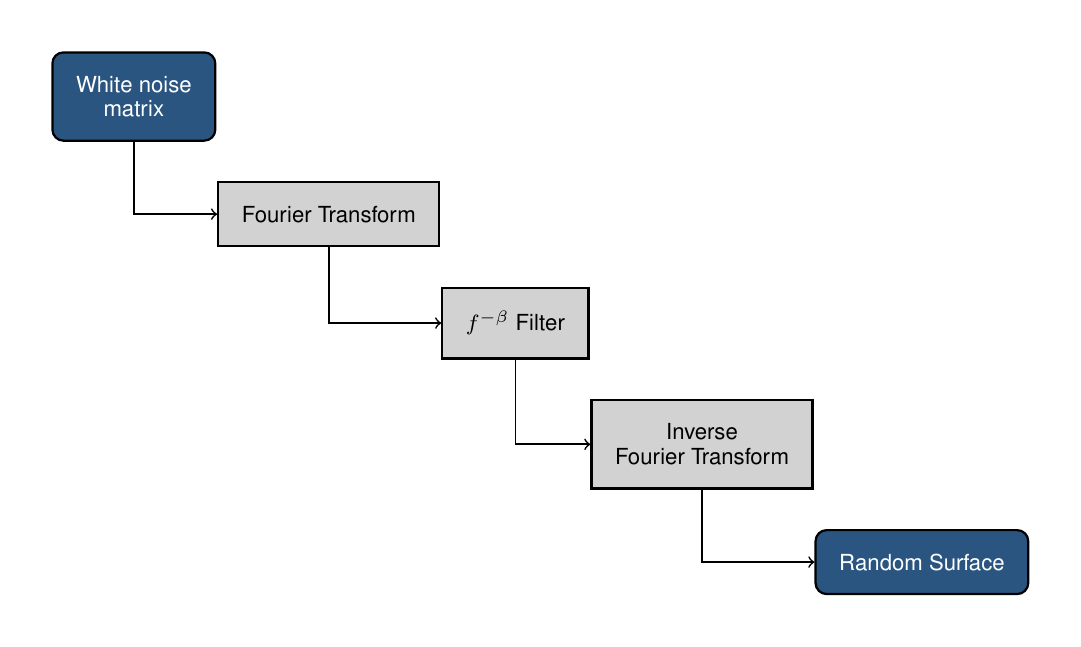
\begin{tikzpicture}[
    		font=\sffamily,
    		every matrix/.style={column sep=0.01cm, row sep=0.5cm},
    		every node/.style={anchor=center, font=\footnotesize, inner sep=.3cm},
    		source/.style={draw, thick, rounded corners, fill={rgb:red,1;green,2;blue,3}, text=white},
    		process/.style={draw, thick, fill=gray!35},
    		to/.style={->,semithick,font=\sffamily\footnotesize}
    		]
    		
    		\matrix[matrix of nodes]
    		{
    			|[source] (1)| \shortstack{White noise  \\ matrix} \\
    			& |[process] (2)| \shortstack{Fourier Transform} \\
    			& & |[process] (3)| \shortstack{$f^{-\beta}$ Filter} \\ 
    			& & & |[process] (4)| \shortstack{Inverse \\ Fourier Transform} \\
    			& & & & |[source] (5)| \shortstack{Random Surface} \\
    		};
    		
    		\draw[to] (1) |- (2);
    		\draw[to] (2) |- (3);
    		\draw[to] (3) |- (4);
    		\draw[to] (4) |- (5);
    		
    		\end{tikzpicture}
    	\end{center}
    	\caption{Fourier Filtering}
    	\label{fig:fourier_filtering}
    \end{figure}		
  
  \subsection{Noise Synthesis} \label{sec:methodology:noise}
  
	\begin{equation}
		\frac{\sum\limits_{i = 0}^{octaves - 1} noise(x \times lacunarity^i + base, y \times lacunarity^i + base) \times persistence^i}{ \sum\limits_{i = 0}^{octaves - 1} persistence^i}
		\label{eq:noise_synthesis}
	\end{equation}
	\myequation{Noise Synthesis}
  
    The noise synthesis method consists on using a weighted average of several random values to approximate an fBm surface, as described in equation \ref{eq:noise_synthesis}. This assumes that the random number generation is a structured noise function. The implementation for this method is based on the code presented in \cite{Musgrave1993}. There are several parameters used in the method, namely:
    
    \begin{itemize}
      \item \textbf{Frequency:} noise arguments divider
      \item \textbf{Number of octaves:} number of noise samples to use
      \item \textbf{Persistence:} contribution gap between successive octaves
      \item \textbf{Lacunarity:} gap between successive frequencies
      \item \textbf{Base:} base value for noise arguments
      \item \textbf{Noise:} noise function used to generate random numbers (eg: perlin noise \cite{Perlin1985}, simplex noise \cite{Perlin2002})
    \end{itemize}
    
    


\section{Phase 3: Blending}  \label{sec:methodology:phase3}
  
  \begin{figure}[!h]
  	\begin{center}
		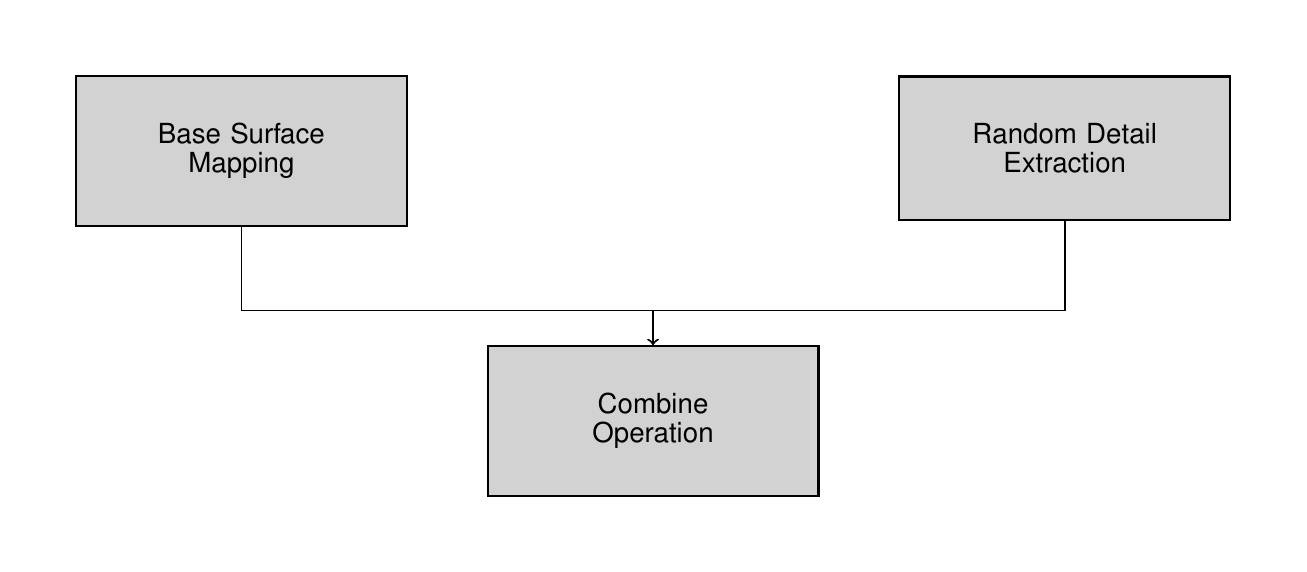
\begin{tikzpicture}[
			 font=\sffamily,
			 every matrix/.style={column sep=1.0cm, row sep=1.5cm},
			 every node/.style={anchor=mid, text centered, font=\normalsize, inner sep=.6cm},
			 process/.style={draw, thick, fill=gray!35},
			 to/.style={->,semithick,font=\sffamily\footnotesize}
			 ]
			 
			 \matrix (table) [matrix of nodes, ampersand replacement=\&]
			 {
				  	|[process, text width = 3.0cm] (base)| \shortstack{Base Surface \\ Mapping} \& \& 
				  	|[process, text width = 3.0cm] (random)| \shortstack{Random Detail \\ Extraction} \\
				  	\& |[process, text width = 3.0cm] (combine)| \shortstack{Combine \\ Operation} \& \\
			 };
			 
			 \draw[to] (base.south) |- (0,1.5) -- (0,1.5) -| (combine.north);
			 \draw[to] (random.south) |- (0,1.5) -- (0,1.5) -| (combine.north);
		
		\end{tikzpicture}
	  \end{center}
 	  \caption{Blending Phase}
 	  \label{fig:blending}
  \end{figure}	
  
  The Blending phase is divided in three parts that are shown in Figure \ref{fig:blending}. 
  
  \subsection {Base Surface Mapping}
  
	In the Base Surface Mapping part the user has the possibility of adjusting the details that will be added to the base surface. This is done by manipulating a spline which represents a function that maps a height value to a multiplier. This mapping is then applied to the base surface generating a multiplier matrix.
	
	The spline function is obtained using a Picewise Monotone Hermite Cubic Interpolation of the control points specified by the user. 
    
  \subsection{Random Detail Extraction}

	In order to extract the details from the random surface, a high-pass filter is used. In the case of this application the HPF is implemented by subtracting a smoothed version of the surface to the surface itself. The smoothed version is obtained by applying a Gaussian Blur filter in frequency domain, using, as cut-off frequency, a value calculated from a user-specified parameter, called Blend Strength, using \ref{eq:cut_off_freq}.
	
	\begin{equation} \label{eq:cut_off_freq}
	  f_{Cut-off} = \frac{0.5}{BlendStrength}
	\end{equation}
	\myequation{Gaussian blur cut-off frequency}
      
  \subsection{Combine Operation}
  
    Using the outputs from the Base Surface Mapping and the Random Detail Extraction parts, the detailed surface can be computed. This is obtained by multiplying the mapped base surface by the random details resulting in an adjusted version of the details. The latter is then added to the Base surface.
      
  \subsection{Result Normalization}
  
	The final step in the blending phase is to normalize the result. This is done using user-defined bounds that need to be comprised between 0 and 255 in order for the surface to be stored in a single channel image using, for each pixel, an 8 bit unsigned integer.
    
  \subsection{Surface Normals Calculation}
  
    In addition to the previously described steps, a normal map is also computed for rendering purposes. This is done by filtering the final surface with a 3 by 3 Sobel filter in both x and y directions.
    
\begin{landscape}
  \pagestyle{lscape}
  
  \section {Parameters Summary}
  \vspace*{\fill}
  
  \begin{table}[h!] \centering \footnotesize
  	 \renewcommand{\arraystretch}{2.0}
  	
     \begin{tabularx}{\linewidth}{|c|c|c|b|c|c|c|}
       \hline
       \multicolumn{2}{|c|}{\textbf{Phase}} & \heading{Name} & \heading{Description} & \heading{Type} & \heading{Minimum} & \heading{Maximum} \\ \hline \hline
       \multirow{6}{*}{\bfseries\shortstack{Random Surface  \\ Generation}} & \textbf{Fourier Filtering} 
       & Filter Power & $\beta$ value & \textit{float} & 1.0 & 2.9 \\ \cline{2-7} 
       & \multirow{5}{*}{\textbf{Noise Synthesis}} 
       & Frequency & Noise arguments divider & \textit{integer} & 1 & 2000 \\ \cline{3-7} 
       & & Octaves & Number of noise samples & \textit{integer} & 1 & 10 \\ \cline{3-7} 
       & & Lacunarity & Gap between successive frequencies & \textit{float} & 0.01 & 10.0 \\ \cline{3-7} 
       & & Persistence & Contribution gap between successive octaves & \textit{float} & 0.01 & 10.0 \\ \cline{3-7} 
       & & Base & Base frequency value & float & 0.01 & 20.0 \\ \hline
       \multicolumn{2}{|c|}{\multirow{2}{*}{\bfseries\shortstack{Blending}}}
       & Spline Control Points & Mapping between original height and detail multiplier. & \textit{float} & 0.0 & 1.0 \\ \cline{3-7} 
       \multicolumn{2}{|c|}{} & Blend Strength & Gaussian Blur control parameter & \textit{integer} & 1 & 500 \\ \hline
       \multicolumn{2}{|c|}{\bfseries\shortstack{Result Normalization}} 
       & Result Bounds & Values between which the final result will be normalized. & \textit{integer} & 0 & 255 \\ \hline
     \end{tabularx}
     \caption{Process Parameters}
     \label{table:parameters}
  \end{table}
  \vspace*{\fill}
\end{landscape}
 
\chapter{Software Architecture} \label{chap:software_architecture}

  \begin{notes}
  	\item Write small introduction about 4+1 architectural view model
  \end{notes}

  \section {Use Case View}
    
    The developed application enables the user to create a detailed terrain from a deterministic base surface. To achieve this goal several features, that aid the user in this process, were implemented. This features are specified in Table \ref{table:user_stories} in the form of user stories. Given the nature of this application only one actor, called User, is needed.
    
    
    \begin{table}[h!]
  \centering
  \renewcommand{\arraystretch}{1.5}
  \begin{tabularx}{\linewidth}{|l|l|b|}
	\hline
    \textbf{Code} & \textbf{Name} & \textbf{Description} \\ \hline
    US-001 & Load Base Surface & As a User I want to load a surface from an image so that I can create a detailed version of it. \\ \hline
    US-002 & Export Result & As a User I want to export the result so that I can use it in other applications. \\ \hline
    US-003 & Add Detail & As a User I want to add detail to a previously loaded base surface. \\ \hline
    US-004 & See Result & As a User I want to see my result as I change the parameters so that I can adjust them more easily. \\ \hline
    US-005 & History & As a User I want to be able to consult a list of previously edited terrains so that I can track my work. \\ \hline
    US-006 & History Parameters & As a User I want to have access to the parameters used in previously edited terrains. \\ \hline
    
  \end{tabularx}
  
  \caption{User Stories}
  \label{table:user_stories}
\end{table}
    
    \subsection {User Interface}
    
      The application was developed using Google's material design \cite{Google2016} for the user interface style. The editor is the main page of the application and it is shown in Figure \ref{fig:editor_page}. It contains a menu bar (1) where the user has access to the available functions, a details panel (2), which has the parameter controllers, a list with the previously results (3), a panel where the details of the selected previous result are displayed (4) and a canvas where the preview of the current current terrain is rendered (5).
      
      \begin{figure}[H]
      	\centering
      	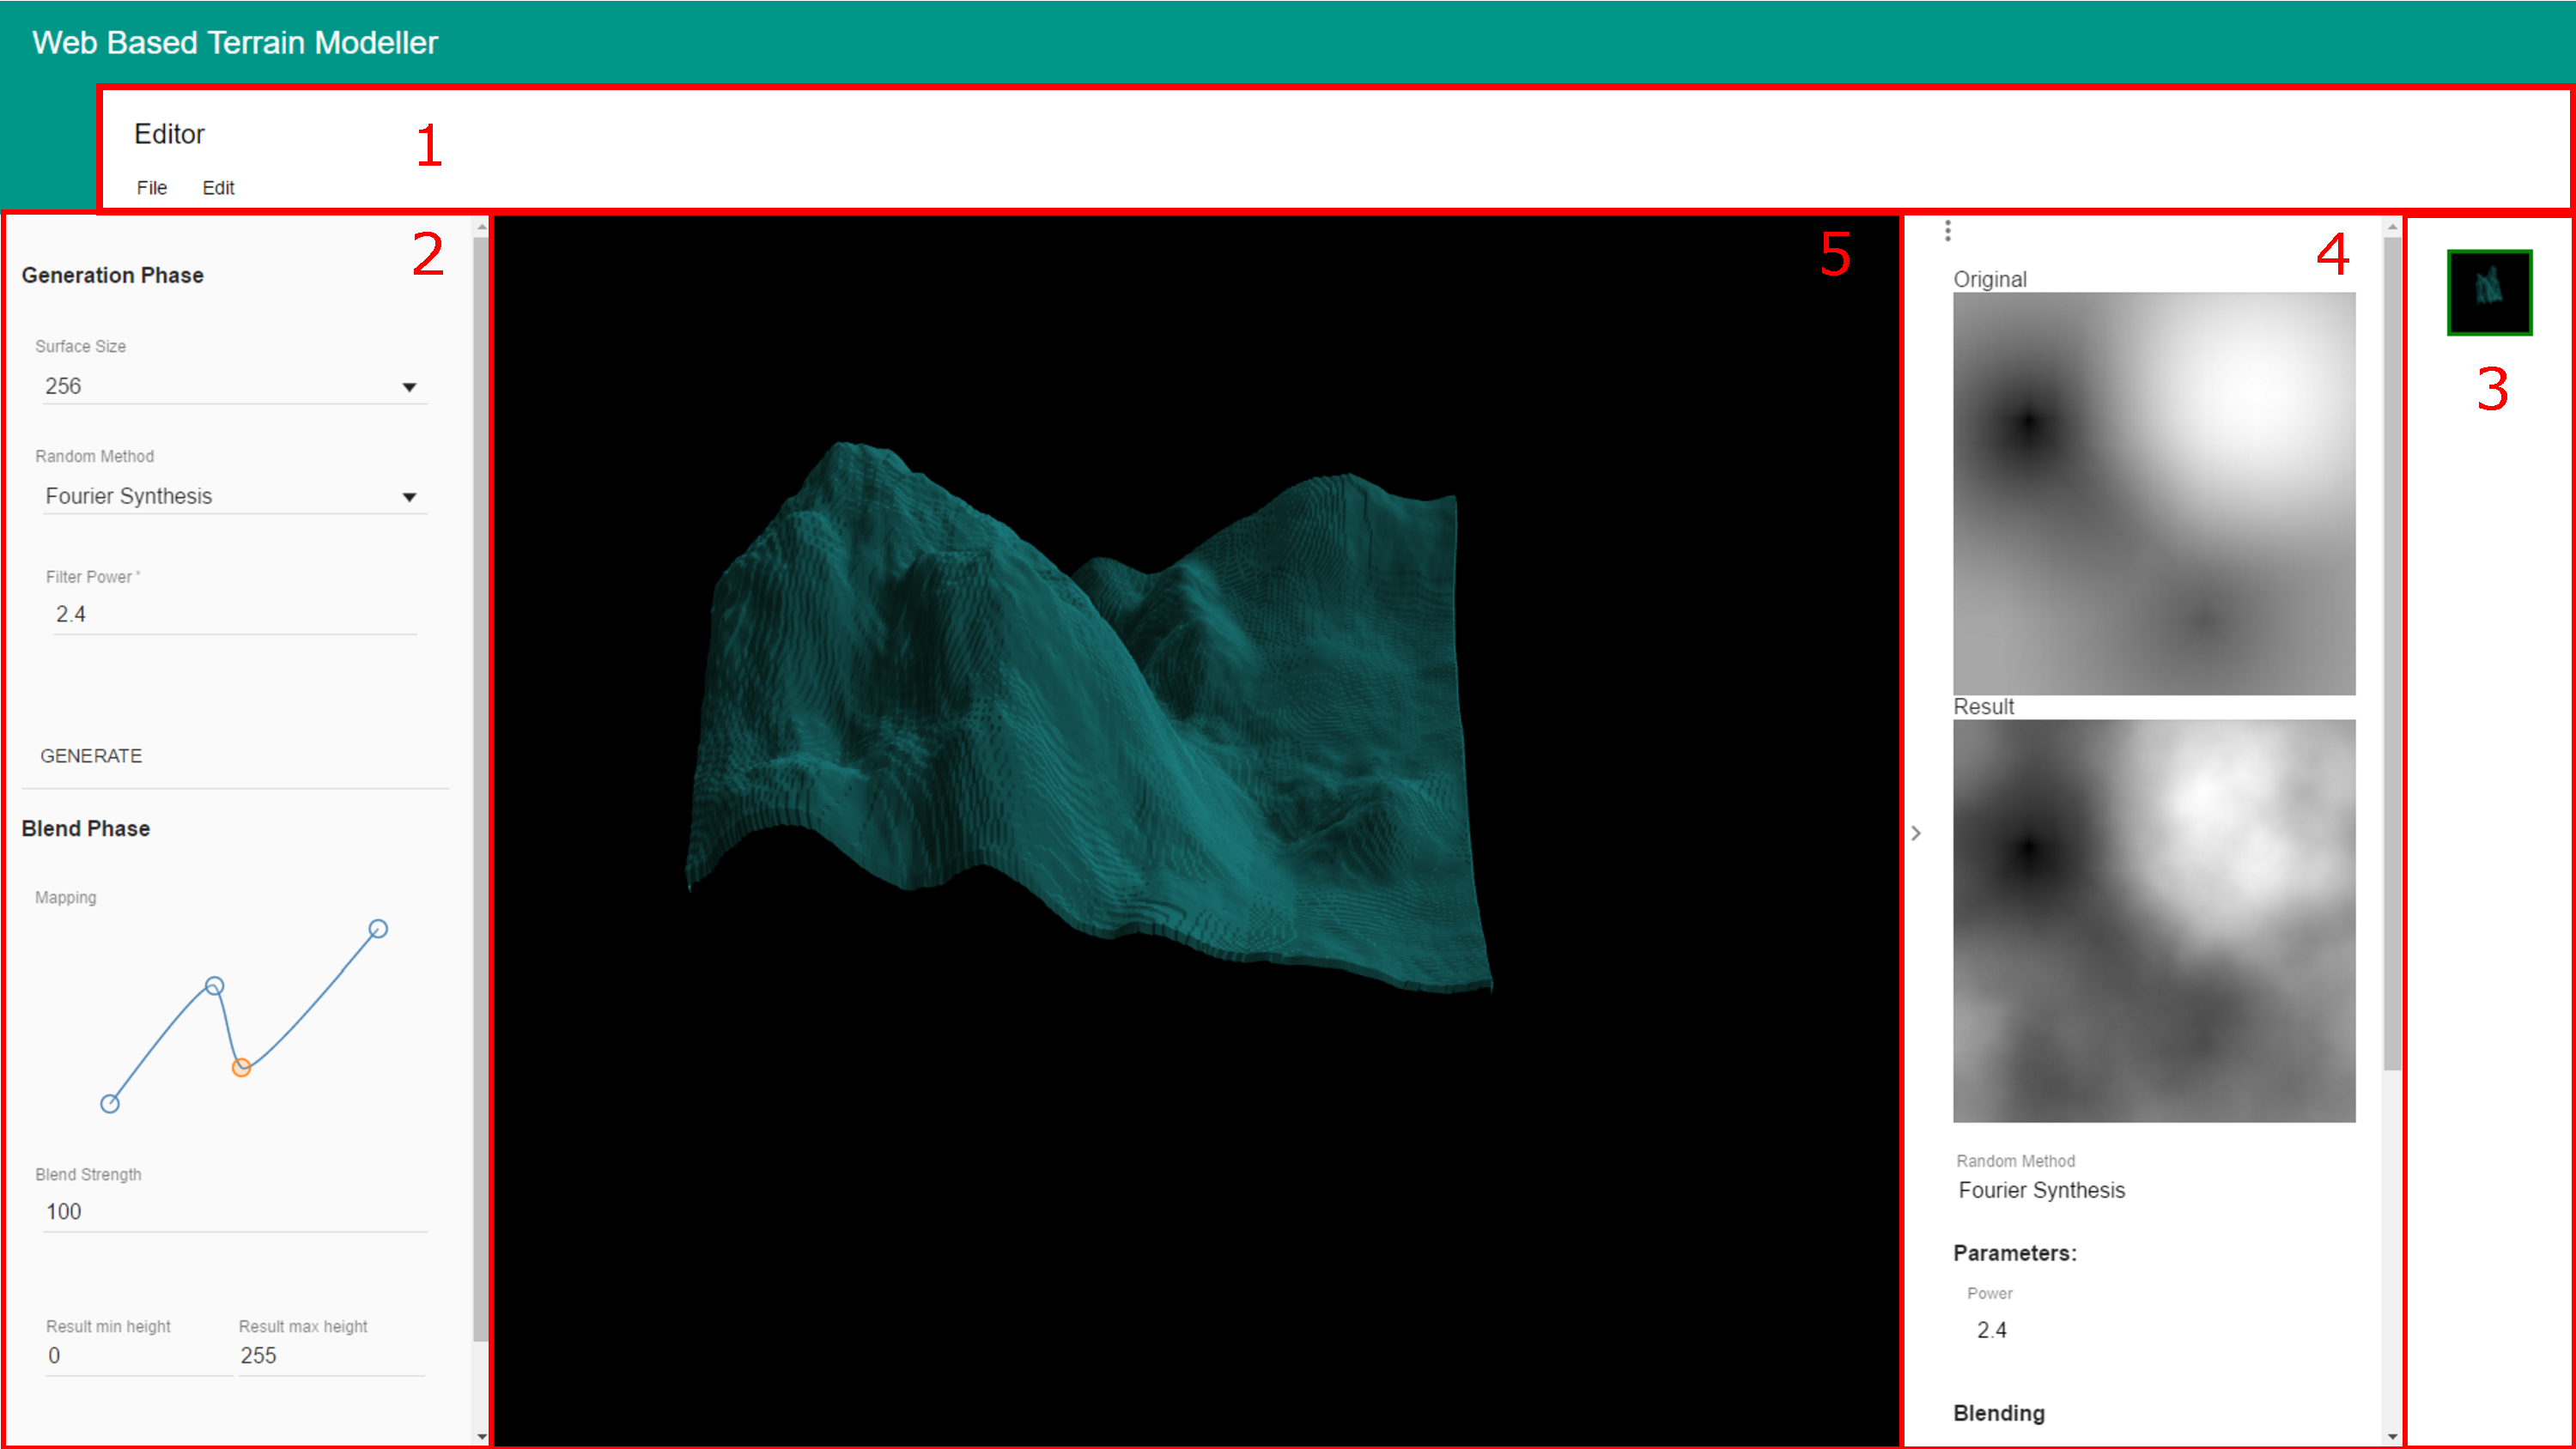
\includegraphics[width=0.95\linewidth]{images/screenshots/editorWithBoxes.pdf}
      	\caption{Editor Page}
      	\label{fig:editor_page}
      \end{figure}
    
    \subsection {Input and Output Formats}
    
      In order to allow the user to load and save his terrains the application implements an import and export feature. The user can either import a Grayscale PNG image, which will be set as the base surface, or import a previously exported Zip file, which will add an entry to the history list and render the result contained in the file. In terms of export formats the user can: obtain: a 4-channel 8-bit per channel PNG containing the height map of the result; a Zip file that can be later imported; and a Grayscale 1-channel 16-bit per channel PNG image of the result height map, which can be import as a landscape in Unreal Engine 4.

  \section {Physical Architecture} %CC Deployment View
    
    The system was developed as a client-side single page web application and thus all the server-side content is static. Given this properties the application works as a static web site and has a simple deployment architecture which consists on a HTTP web server and a web browser, as shown in Figure \ref{fig:deployment_diagram}.
    
    \begin{figure}[h!]
    	\begin{center}
    		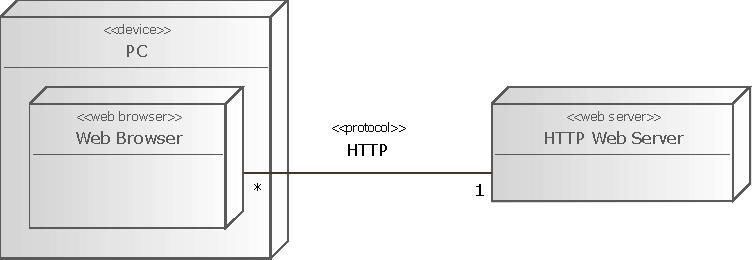
\includegraphics[width=0.9\textwidth]{images/diagrams/deployment.pdf}
    	\end{center}
    	\caption{Deployment Diagram}
    	\label{fig:deployment_diagram}
    \end{figure}
    
  \section {Implementation Architecture} %CC Implementation View
    
    The application is composed by three submodules (Figure \ref{fig:component_diagram}). The \textit{components} submodule is responsible for configuring the page routing and, as such, contains, as submodules, the editor and the benchmarks pages. The \textit{common} module contains services and directives that are generic to the application. The \textit{imgproc} module contains the image processing utilities.
    
    \begin{figure}[H]
      \begin{center}
      	 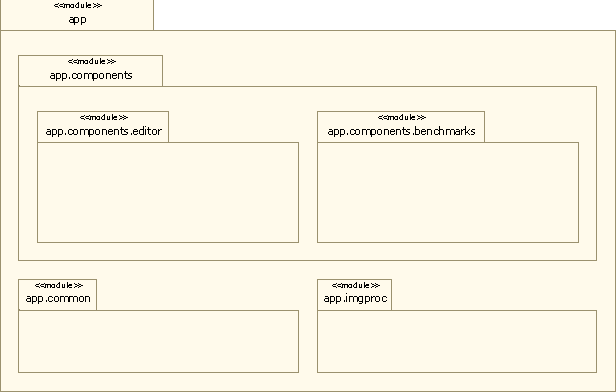
\includegraphics[width=0.9\textwidth]{images/diagrams/component.pdf}
      \end{center}
      \caption{Component Diagram}
      \label{fig:component_diagram}
    \end{figure}
    
    \begin{notes}
    	\item Fill Component Diagram modules with classes.
    \end{notes}

    \subsection {Technologies}    
      
      Given the web-based requirement the application needed to be in Javascript. For convenience the Babel transpiler was used so that the development could be done in ECMAScript 6, which is a newer standard of Javascript. Additionally, to simplify the management of the required dependencies, JSPM and System.js were used, which, integrating with Babel, enable better support for ECMAScript 6 modules. 
      
      To aid the development of the application, Angular.js was used. This framework implements the MVC pattern, which was used to better modularize the source code.
      
      The terrain viewer was implemented using three.js, which is a 3D rendering Javascript library that allows the developer to create 3D Scenes in a straight forward way. 
      
      In order to parallelize some operations, WebGL 2.0 was used. This implementation will be detailed in section \ref{sec:software:process:gpu}
    
  \section {Logical View} %CC Logical View
  
	  The logical architecture of the developed application was influenced by the usage of Angular.js. Due to this in Figure \ref{fig:class_diagram}, where the UML class diagram for the application is shown, two prototypes are attributed to the classes: controller and service; the controller classes are responsible by the dynamic behaviour of the element to which they are attributed; the service classes are lazily instantiated singletons that are injected in the application in the required modules.
    
      \begin{figure}[H]
    	\begin{center}
    	  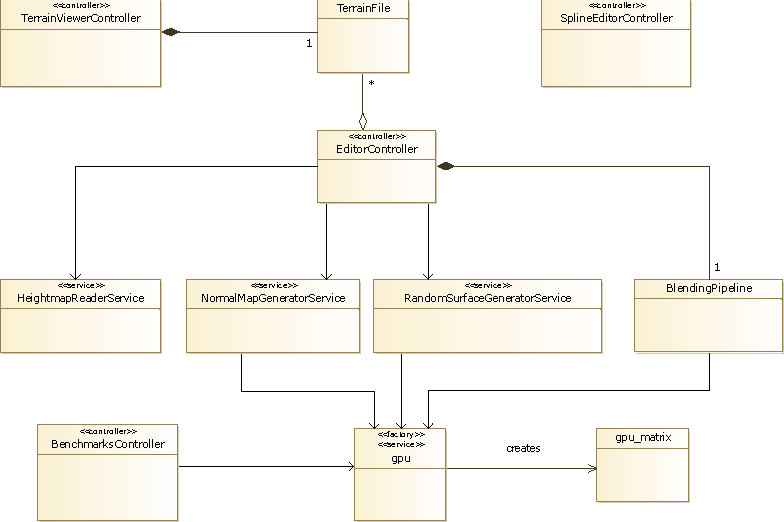
\includegraphics[width=\textwidth]{images/diagrams/class.pdf}
    	\end{center}
    	\caption{Class Diagram}
    	\label{fig:class_diagram}
      \end{figure}
      
      \begin{notes}
      	\item Fill Class Diagram with main class methods
      \end{notes}
    
  \section {Process View}
    
    \subsection {GPU Computation Framework} \label{sec:software:process:gpu} %CC Process View
    
      In order to optimize some operations performed by the application a GPU computation framework was implemented. This framework uses WebGL 2 to perform pixel-wise operations on images. WebGL 2 is a 3D rendering API for the web derived from OpenGL ES 3.0, which features a programmable rendering pipeline that gives the developer the ability to manipulate the rendering data in two different stages: the vertex stage and the fragment stage. The vertex stage executes the vertex shader using as input the vertex data and it outputs the final vertex position as a 4-component floating-point vector in homogeneous coordinates $(x, y, z, w)$. In the fragment stage the fragment shader is executed once per fragment and it's output depends on the active render target, which can be either the HTML canvas or a texture. When the render target is the HTML canvas the output is 4-component floating-point vector that represents the color of the fragment. When the render target is a texture the output depends on the texture format. For a texture to be a render target it's format needs to be \textit{color-renderable} and, in WebGL 1, as in OpenGL ES 2, only 3 or 4 component integer textures are \textit{color-renderable}. This limitation is surpassed in WebGL 2 and in OpenGL ES 3, where, with the \textit{EXT\_color\_buffer\_float} extension, floating-point textures with 1, 2, 3 or 4 components are considered \textit{color-renderable}.
      
      In order to use WebGL for computations the framework uses a texture as the render target and renders a square on a viewport of the same size as the texture, resulting in a 1:1 fragment to pixel mapping, and uses a specific fragment shader depending on the algorithm that is being executed. 
      
      \subsubsection{Implementation Details}
      
        To implement this framework two classes were created: the gpu class and the gpu\_matrix class (Figure \ref{fig:class_diagram}). The gpu class works as an Angular.js service which is injected wherever it is needed. At the same time this class is also factory for gpu\_matrix class instances, as the latter need an initialized gpu instance to be created, this is noted in the class diagram by the usage of the \textit{factory} prototype and the \textit{creates} relation between the two classes.
        
        The gpu\_matrix class represents a matrix that was uploaded to the GPU. Due to restrictions imposed by WebGL the textures dimensions need to be powers of 2 and their format is limited to 1, 2 or 4 components per pixel and 8 bits unsigned integer, 32 bits signed integer or 32 bits floating-point components. This class handles the allocation and reallocation of the textures and framebuffers, as well as, the upload and download of the matrix to and from the GPU device.
        
        The gpu class also contains the methods to execute the algorithms. Although this methods have different parameters depending on the algorithm that they execute, they all have as last parameter the return variable, which is also returned by the function. This rule enables the framework to reuse gpu\_matrix instances when one is passed into a function, otherwise, that is, when the last parameter is \textit{undefined}, a new gpu\_matrix is created and returned. Additionally, given that each algorithm requires different shader programs, a lazy initialization for the shader programs was implemented. This feature results in a smaller initialization time as it only compiles the shader programs when they are needed, on the first time a certain function is called.
      
	  \subsubsection{Implemented algorithms}
	  
	    The implemented algorithms can be divided in 3 categories:
	    \begin{itemize}
	      \item Fast Fourier Transform
	      \item Element-wise Operations
	      \item Matrix Normalization
	    \end{itemize}
	    
	    The Fast Fourier Transform was implemented using the radix-2 Stockham FFT algorithm used in \cite{Lloyd2008}. This algorithm avoids the bit reversal phase of the FFT by reordering the dataflow and, consequently, cannot be performed in-place, which is not a problem for this implementation taking into account that textures in WebGL cannot be read from and written to at the same time. Additionally, as noted in \cite{Lloyd2008}, in order to compute a 2D FFT, the matrix is usually transposed to optimize the traversal of an array stored linearly in memory. This issue is also surpassed as, on a GPU, textures are swizzle, thus, no transposes are performed. 
	    To implement the Inverse Fast Fourier Transform the FFT implementation was used with the real and imaginary parts swapped as shown in \cite[p.450]{Lyons2004}.
	    
	    The element-wise operations implemented are addition, subtraction, multiplication and division. There are two version of this operations: the binary version, where two matrices are combined using the given operator, and the immediate version, where the operator is applied to matrix and to a given value. Additionally some image processing algorithms were implemented: two frequency domain filters: the gaussian blur and the $f^{-\beta}$, that were implemented by multiplying the fourier transform of the matrix by the fourier transform of the filter, which was computed using the analytical formulas; and a spatial domain sobel filter, both in x and y, which was implemented by performing a pixel-wise convolution of the matrix.
	    
	    In order to implement matrix normalization the process was divided in two phases. The first phase consists in finding the minimum and the maximum value of the matrix. The second is the element-wise execution of equation \ref{eq:software:gpu:norm}. To implement the first phase in parallel a reduction method was used. This method consists in first reducing each row to it's minimum and maximum, resulting in a vector of two values, and then reducing the resultant vector two the global minimum and maximum of the matrix.
	    
	    \begin{equation} \label{eq:software:gpu:norm}
		  M_{Normalized}(x, y) = \frac{M(x, y) - minimum_M}{maximum_M - minimum_M}
	    \end{equation}
	    \myequation{Normalization Operation}
	    
    \subsection {Blending Process Pipeline} %CC Process View
      
      In order to improve the application's performance a pipeline for the blending process was created. This pipeline saves the intermediate matrices of the blending process and reuses them when a parameter changes. This process is illustrated in the activity diagram shown in Figure \ref{fig:activity_blending_process}, where the initial nodes represent the starting point when the associated parameter is modified. When this process reaches the final node a callback is invoked to trigger an update in the user interface.
      
      \begin{figure}[h]
      	\begin{center}
      	  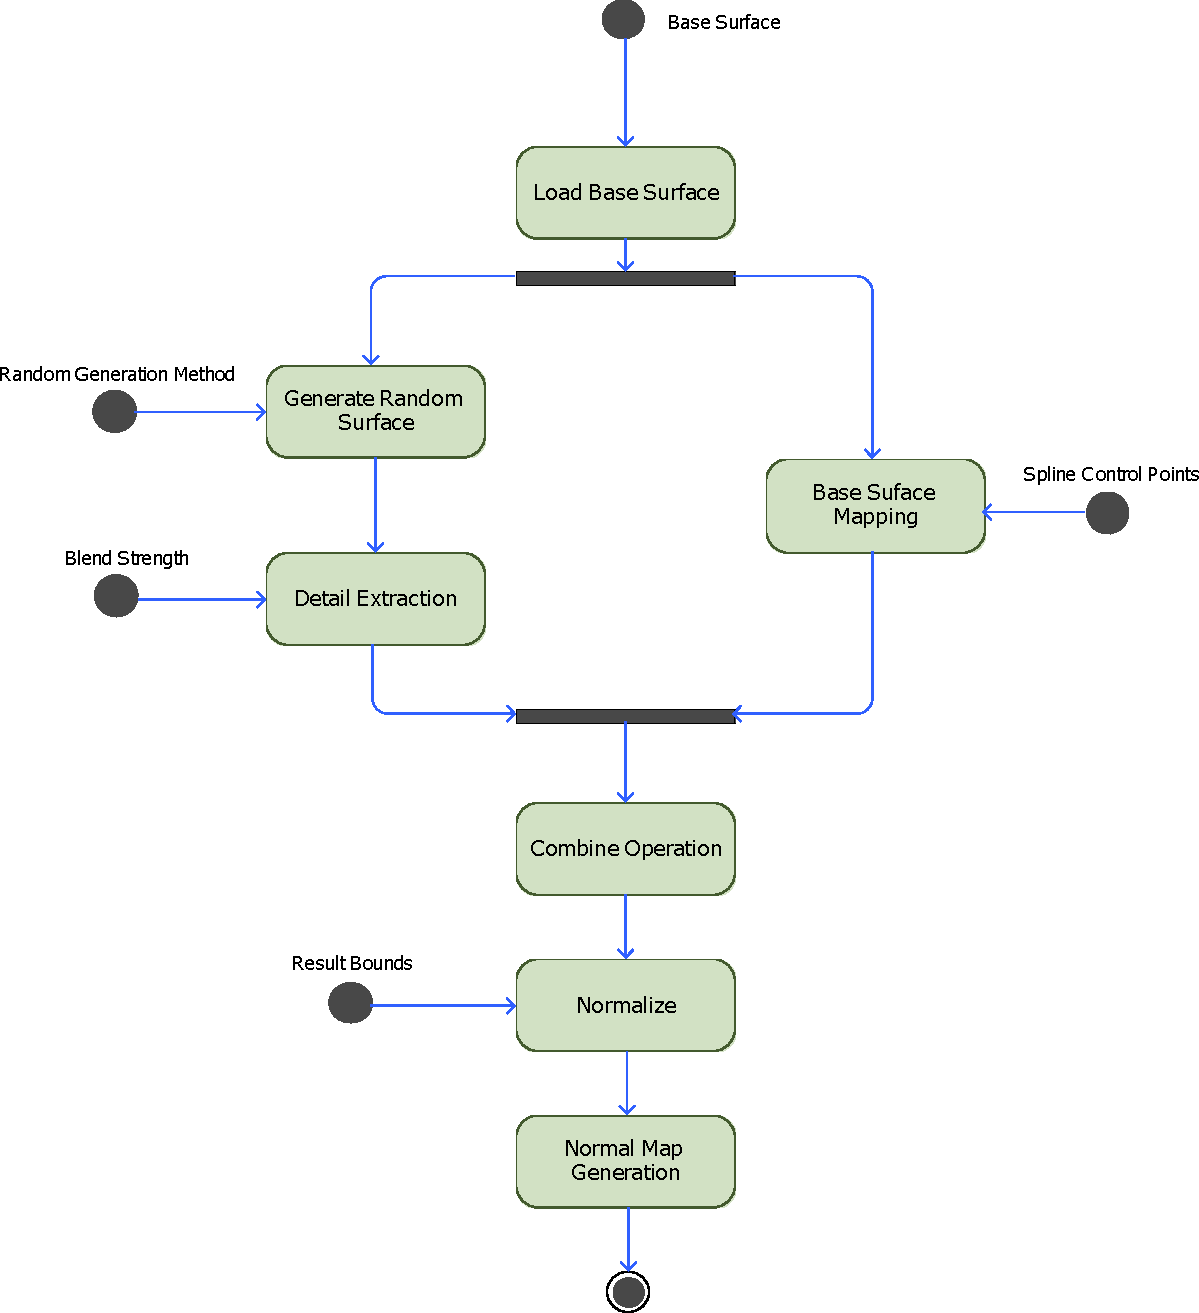
\includegraphics[width=0.98\textwidth]{images/diagrams/blending_process.pdf}
      	\end{center}
        \caption{Activity diagram for the blending process}
        \label{fig:activity_blending_process}
      \end{figure} 
      
\chapter{Results} \label{chap:results}

  \section {Visual Presentation} % Before and After
  
    \begin{notes}
      \item Show some comparison between base surfaces and results with different parameters
      \item Show some unreal engine 4 renderings of the results
    \end{notes}
  
  \section {GPU vs CPU Computations Benchmarks}
  
    \begin{notes}
      \item Hardware Specification
      \item Software Specification (including chrome version and flags)
      \item Operations/second or time comparison
      \item Ratios
    \end{notes}
\chapter{Conclusions}


% References - you can use BiBTeX inside the 'references' environment if you want.
% For short reference lists, you might find it just as easy to use the bibitem form.
\begin{references}
	\bibitem{Mandelbrot1983} 
Mandelbrot BB. The Fractal Geometry of Nature. 1983.

\bibitem{Mandelbrot1968} 
Mandelbrot BB, Ness JV. Fractional Brownian motions, fractional noises and applications. SIAM review. 1968; Available at: http://epubs.siam.org/doi/abs/10.1137/1010093

\bibitem{Musgrave1993} 
Musgrave FK. Methods for Realistic Landscape Imaging. Thesis. Yale University; 1993. pp. 1--276. Available at: http://www.kenmusgrave.com/dissertation.pdf

\bibitem{Ebert2003} 
Ebert DS, Musgrave FK, Peachey D, Perlin K, Worley S, Mark WR, et al. Texturing and Modeling. Texturing and Modeling. Elsevier; 2003. 9 p. Available at: DOI:10.1016/B978-155860848-1/50050-4

\bibitem{Musgrave1989} 
Musgrave FK, Kolb CE, Mace RS. The synthesis and rendering of eroded fractal terrains. ACM SIGGRAPH Computer Graphics. New York, New York, USA: ACM Press; 1989; 23(3): 41--50. Available at: DOI:10.1145/74334.74337

\bibitem{Mandelbrot1988} 
Mandelbrot BB. Fractal landscapes without creases and with rivers. The science of fractal images. 1988. pp. 243--260. Available at: http://dl.acm.org/citation.cfm?id=61160 http://portal.acm.org/citation.cfm?id=61160

\bibitem{Fournier1982} 
Fournier A, Fussell D, Carpenter L. Computer rendering of stochastic models. Communications of the ACM. ACM; June 1982; 25(6): 371--384. Available at: DOI:10.1145/358523.358553

\bibitem{Lewis1987} 
Lewis JP. Generalized stochastic subdivision. ACM Transactions on Graphics. 1987; 6(3): 167--190. Available at: DOI:10.1145/35068.35069

\bibitem{Miller1986} 
Miller GSP. The definition and rendering of terrain maps. ACM SIGGRAPH Computer Graphics. 1986; 20(4): 39--48. Available at: DOI:10.1145/15886.15890

\bibitem{Saupe1988} 
Saupe D. Algorithms for random fractals. The Science of Fractal Images. New York, NY: Springer New York; 1988. pp. 71--136. Available at: DOI:10.1007/978-1-4612-3784-6\_2

\bibitem{Voss1985} 
Voss RF. Random Fractal Forgeries. Fundamental Algorithms for Computer Graphics. Berlin, Heidelberg: Springer Berlin Heidelberg; 1985. pp. 805--835. Available at: DOI:10.1007/978-3-642-84574-1\_34

\bibitem{Perlin1985} 
Perlin K. An image synthesizer. ACM SIGGRAPH Computer Graphics. 1985; 19(3): 287--296. Available at: DOI:10.1145/325165.325247

\bibitem{Perlin2002} 
Perlin K. Improving noise. ACM Transactions on Graphics. New York, New York, USA: ACM Press; 2002; 21(3): 2--3. Available at: DOI:10.1145/566654.566636

\bibitem{Spencer2015} 
Spencer K. OpenSimplexNoise.java. 2015. Available at: https://gist.github.com/KdotJPG/b1270127455a94ac5d19

\bibitem{Musgrave1994} 
Musgrave FK. 2 Procedural Fractal Terrains. Texturing and Modelling. A Procedural approach. 1994;  2.

\bibitem{Evertsz1992} 
Evertsz CJG, Mandelbrot BB. Multifractal measures. Chaos and Fractals. 1992. pp. 921--953. Available at: http://lipenreferences.googlecode.com/svn/trunk/Papers/Multifractals/1992Multifractal Measures.pdf

\bibitem{Google2016} 
Google. Material design. Google design guidelines. 2016. Available at: https://material.google.com


\end{references}

%% Back matter
%
% This is where we include appendices and references

\chapter*{Appendices}
\addcontentsline{toc}{chapter}{Appendices}

Whilst Heading 1 to Heading 6 can be used to number headings in the main body of the thesis, Heading styles 7–9 have been modified specifically for lettered appendix headings with Heading 7 having the ‘Appendix’ prefix as shown below. \\

\begin{appendices}	
	\section{User Manual}
\subsection {User Section 1}
    \subsubsection {User Subsection 1}
    Something
    
\subsection {User Section 2}

\section{Appendix 2}

\subsection{Appendix Section 2}
\end{appendices}

\backmatter

\end{document}

